\subsection{A Model for DevOps Adoption and its Application}\label{sec:case_study}

Based on H1-H4 hypothesis, we present a three step model that
explains how to adopt DevOps according with our understanding. The
model considers the following steps:
\begin{itemize}
\item In the first step, a company should
disseminate that the goal with a DevOps adoption should be
the establishment of a \cc between
development and operations teams.

\item In the second step, a company should select and develop
the most suitable enablers according with its context. The enablers
are means commonly used to develop the \cat{collaboration culture}
and its concepts.

\item In the third step, a company should check the outcomes of the
DevOps adoption in order to verify the alignment with
industrial practices and to explore them according to the
need of the company.
\end{itemize}

%% \begin{figure*}[t]
%%   \centering
%%     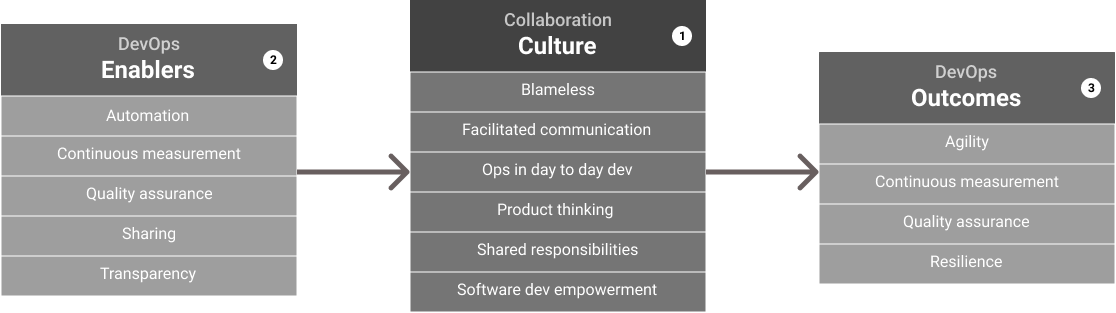
\includegraphics[width=14.26cm,height=4cm,natwidth=1116,natheight=313]{model.png}
%%     \caption{DevOps Adoption Model}
%%     \label{fig2}
%% \end{figure*}


Our proposed model has been applied to guide the DevOps adoption at the Brazilian Federal Court of
Accounts (TCU). TCU is responsible for the accounting, financial, budget, performance, and property
oversight of federal institutions and entities of the country. Currently, there are 2500
professionals working at TCU, of which approximately 300 work directly on either
software development or operations. The source code repository at TCU hosts more then 200 software projects, totaling
over 4 million lines of code.

Before the application of our model, TCU has produced some results w.r.t deployment
automation and the focus was being directed to the tooling issue. Considering this
old-fashioned perspective of DevOps, the conflicts between development and operations
teams continued. That is, the mere advance in implanting ``DevOps tools" simply
changed the points of conflict, but they persisted.

After the presentation of our  model in a series of lectures, development and
operations teams changed their focus to build a collaboration culture. This
change was only possible due to the engagement and sponsorship of the IT
managers. Looking to the concepts within collaborative culture category, the first practical
action at TCU was to facilitate communication between teams. The use of tickets
was then abolished. The problems had to be solved in a collaborative way, preferably
face to face. In cases where face to face communication was not feasible,
communication tools that allowed direct contact should be used instead.

Looking to enablers, TCU is applying \cat{sharing and transparency} concepts.
The role of internal tech talks and committees to disseminate that collaboration
culture and related concepts is being reinforced.
When a new infrastructure had to be provided and configured, the current guideline is
that it must exist a kind of \emph{pair programming} between developers and infrastructure
members. All application related tasks must be executed in a collaborative
way. Naturally, the professionals noticed that automation would facilitate the
operationalization of that collaboration. For this reason, the infrastructure provisioning
and management was automated. Also w.r.t  the \cat{sharing and transparency} category,
the use of shared pipelines to contain this automation procedures was set as default.

TCU also uses continuous measurement and quality assurance concepts as
enablers of its DevOps adoption. The applications started to be continuously
tested and measured. The tests were automated and included in the pipelines.
Verification of test coverage and quality code also became part of the pipeline.
This increased the confidence between teams. With more confidence, TCU started
to explore the potential of DevOps tools, like recovery automation, zero
down-time, and auto scaling. The deployment has been also automated.

Before DevOps, deployment activities were historically a controversial point at TCU.
Several conflicts occurred over time. Rigid procedures were created to try to
avoid problems. These ``rigid procedures'' often led to periods of months
without any software delivery. The more collaborative scenario, with strong appeal in automation and quality,
created by following an appropriate path in adopting DevOps, enabled the deployment activities to became
a lightweight task at TCU. Continuous deployment became a reality and currently several deployments
occurs as regular activities of the development teams at TCU.

Since TCU is a government institutions, some advances in DevOps adoption still comes up
against regulatory issues. For example, there are internal regulations that
establish that only the operations sector is responsible for issues related to
application infrastructure, contrasting with shared responsibilities that is
part of collaboration culture. Nevertheless, our model enabled TCU to adopt DevOps in a more
sustainable way. Knowing the role
of each DevOps element in the adoption was fundamental for TCU to avoid points
of failure and to build a collaborative environment that supports the
exploitation of DevOps benefits in the long run.
